\documentclass[sigconf, anonymous]{acmart} %use acmart_mod for handin
% NOTE: To make the documnet anonymous, use the command \documentclass[sigconf, anonymous]{acmart}
%
%% \BibTeX command to typeset BibTeX logo in the docs
\AtBeginDocument{%
	\providecommand\BibTeX{{%
		\normalfont B\kern-0.5em{\scshape i\kern-0.25em b}\kern-0.8em\TeX}}}

\usepackage{lipsum}
\usepackage{graphicx}
\usepackage{tikz}
\usetikzlibrary{arrows.meta}
%% Rights management information.  This information is sent to you
%% when you complete the rights form.  These commands have SAMPLE
%% values in them; it is your responsibility as an author to replace
%% the commands and values with those provided to you when you
%% complete the rights form.
\copyrightyear{2024}
\acmYear{2024}
\setcopyright{rightsretained}
\acmISBN{N/A}
\acmDOI{N/A}

%% These commands are for a PROCEEDINGS abstract or paper.
\acmConference[CMPUT 302 '24: Illumia Labs]{}{January 2024}{Edmonton AB}

% shorthand for ualberta definition
\newcommand{\ualberta}{
	\affiliation{%
	  \institution{the University of Alberta}
	  \city{Edmonton}
	  \state{Alberta}
	  \country{Canada}
	}
}

\begin{document}
	%%
	%% The "title" command has an optional parameter,
	%% allowing the author to define a "short title" to be used in page headers.
	\title{Illumia Labs \textit{Scenario Builder} Discount Evaluation}
	
	%% The "author" command and its associated commands are used to define
	%% the authors and their affiliations.
	%% Of note is the shared affiliation of the first two authors, and the
	%% "authornote" and "authornotemark" commands
	%% used to denote shared contribution to the research.
	\author{Ayrton Chilibeck}
	\authornote{All authors contributed equally to this research, and are listed in alphabetical order for simplicity}
	\email{achilibe@ualberta.ca}
	\ualberta

	\author{Eric Kim}
	\authornotemark[1]
	\email{dek@ualberta.ca}
	\ualberta

	\author{Yu Liu}
	\authornotemark[1]
	\email{yliu30@ualberta.ca}
	\ualberta
	
	\author{Vedant Talati}
	\authornotemark[1]
	\email{vtalati@ualberta.ca}
	\ualberta

	\author{Marcus Wilson}
	\authornotemark[1]
	\email{mawilso1@ualberta.ca}
	\ualberta

	%%
	%% By default, the full list of authors will be used in the page
	%% headers. Often, this list is too long, and will overlap
	%% other information printed in the page headers. This command allows
	%% the author to define a more concise list
	%% of authors' names for this purpose.
	\renewcommand{\shortauthors}{Chilibeck, Kim, Liu, Talati, Wilson}
	
	%%
	%% The abstract is a short summary of the work to be presented in the
	%% article.
	\begin{abstract}
	  We analyze the functionality and quality of Illumia Lab's \textit{Scenario Builder} to comment on potential improvements and provide a short-term roadmap for development and improvement of the application. We encounter and provide solutions for various problems in the UI, the functionality of the system and the documentation of the program with respect to Human-Computer Interaction principles, Gestalt principles and CRAP design principles. Our solutions follow previously established results from the field of HCI, colour theory as well as results from our experiences as users.
	\end{abstract}

	\keywords{Human-Computer Interaction, UX Design}
	
	\maketitle
	
\section{Introduction}
We evaluated the Illumia Lab's \textit{Scenario Builder} for
\section{System Flaws}\label{sec:flaws}
During our exploration and use of the system, we encountered problems in the UI, the program functionality and the documentation of the program. We outline the most important findings in the following sections.
\subsection{UI}
Our results from UI analysis are largely cosmetic, but the current state of the software impedes effective use of the system by the end users. The layout of the system does not efficiently show the information in a given scene and the process of changing a scene takes a large amount of work from the user. Additionally, the system does not have clear indication of the correct user actions and fails to introduce the user to the potential actions at any given point in the scene building process.

\subsubsection{Colour-Scheme}
The current colour scheme (Purple (\verb|#07012F|), Blue (\verb|#0191FD|) and Red (\verb|#FC5C00|)) is jarring to the eyes. The literature establishes that red and purple are particularly hard for users to look at for extended periods of time~\cite{jonesHumancomputerInteractionDesign1989}. Some users may prefer a more darker or lighter color scheme and the interface could benefit from a light and dark mode. Furthermore, there are instances where red is used as the colour for the program's desired state when presented with multiple choices. This may have confusing implications towards the user as red is often associated with being a 'negation' or 'emergency' choice when that is not the intention.

\subsubsection{Tab Display}
The current display of tabs in the scene builder fails to effectively show the user the state of the program. Tabs for each scene do not give the user context on the scene's purpose or the information contained therein. The preview pane attempts to mitigate these shortcomings, but the scene-graph display is lacking in relationships to other scenes.

\subsubsection{Preview Pane}
The alignment in the preview pane is poor, in addition to an absence of dynamic sizing of the screen (for mobile and re-sizable web pages) the utility of the data presented is questionable.

\subsubsection{Ease of Use}
Building a scene currently takes a minimum of 9 clicks. Although the community has debunked the '3-click rule'~\cite{ThreeclickRule2023}, the importance of ease of access for information is still paramount in design. Current research into the concept of 'Interaction Elasticity' \cite{experienceInteractionElasticity} rather enforces the significance of eliminating useless interaction. Currently, the scene builder presents the user with a great deal of useless interaction in the form of these clicks.

\subsection{Functionality}
The website currently has a number of usability-impacting, unimplemented features. We list the systems impacted here.

\subsubsection{Saving}
Currently, the system does not allow for saving of a scene or working on a previously saved scene. This prevents the user from creating a well-though-out, well-crafted scene.

\subsubsection{Avatar}
The use of an avatar does not feel necessary to the development of a scene,  and the stated requirement in the builder is not reflected in the business logic.

\subsection{Documentation}
In general, the builder lacks documentation. A number of terms and interactions with the software are not explained by the user's interactions with the program.

\section{Remediations}\label{remediations}
We propose a number of possible solutions to the problems mentioned above that will improve the usability of the application and touch on additional, smaller problems that we neglect to mention in this report, but are nonetheless important.

\subsection{UI}
\begin{figure}
  \begin{center}
  \includegraphics[scale=0.5]{media/sidebar.png}
  \end{center}
\caption{A prototype sidebar navigation system.}\label{fig1}
\end{figure}
We suggest a sidebar-based UI such as pictured in Figure \ref{fig1}. This UI paradigm will provide the user with more information on any given scene in the program and allow the user to recognize the full state of the program at a glance without wading through screen after screen of data.

When combined with an information page for the selected screen (or the graph view of connections between scenes), we can give the user a more granular view of the data. It is important to note that this type of modification is an overhaul of the frontend design for the website, so the transition will not be easy but the application of this type of UI is well loved in modern UI design~\cite{YourConnectedWorkspace} \cite{SupabaseOpenSource} \cite{FlutterBuildApps}. Adding the flexibility for the user to navigate to any scene in a single click will then reduce useless interaction with the program, bettering the user experience.

This type of UI will also make user error handling more visible to the user. Instead of using the single exclamation point, we can highlight all the fields invalid data in the associated page and provide a clear message to the user with respect to the nature of their violations all on one screen. We can also highlight the issues in all scenes by highlighting nodes on the sidebar as required. This way, the user does not need to chase every bug individually and can rather see where every bug is without having to perform trial and error modifications.

\subsubsection{The Scenarios Folder}
You will notice in the mockup that we have added a scenarios folder, this serves to give the user a space to switch between different scenarios they are beginning to develop and possibly to store other scene elements they use frequently. This will require the implementation of the saving system, but will improve the user's ability to reuse gode as required.

\subsubsection{Log Out}
The sidebar also contains a Log-Out button, it is assumed that eventually the avatar will be associated to the user in order to create some kind of account for the user to log in and out with. This would be an easy way to implement this feature.

\subsubsection{The Scenario Page}
\begin{figure*}
  \begin{center}
	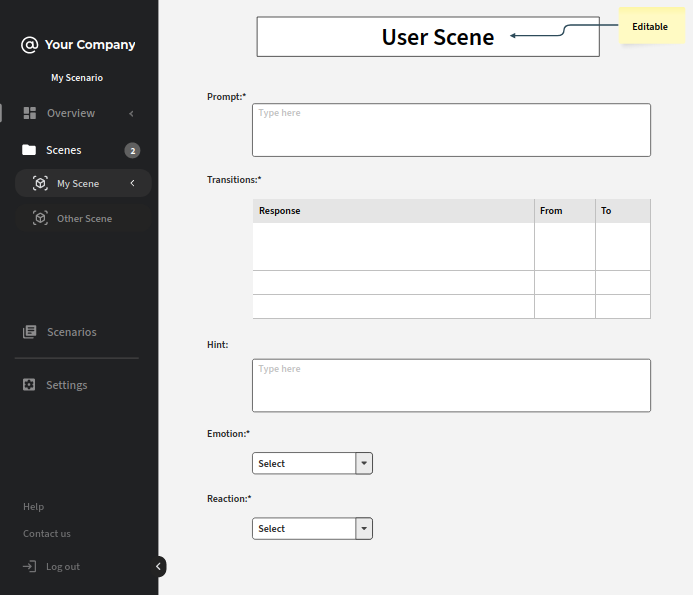
\includegraphics[scale=0.5]{media/Scene_Page.png}
  \end{center}
\caption{A mockup of a scene page for editing individual scenes in the program}\label{fig2}
\end{figure*}
The accompanying scenario page shown in Figure \ref{fig2} will give the user the options to input all necessary data and efficiently view all of their options. This will provide a visual interface for the user to modify their scene without added interaction.

Additionally, there is the option to outline the elements in red or some other colour to indicate a non-conforming piece of data. In the tab like display, the user is not aware of the exact location of flaws in their data.

We could also implement a dropdown in the sidebar in each scene tat gives a short summary of the data entered and can also indicate errors in the data entry. This will give users an even more general view of their scene.

\textbf{Note}: We are unsure of the difference between the emotion and reaction elements. The two descriptions seem to be linked, and as such we wonder if the program could eliminate one or the other.

\subsection{Functionality}
With the implementation of a sidebar navigation paradigm, we can eliminate the need for a lot of the confusing actions that were present in the tab layout. This includes the arrows above the tabs and the delete button (which could now be placed on the sidebar element or in its dropdown menu), as well as a myriad of alignment problems. Now the data has one single point of control that can be stored as one object for manipulation and viewing.

\subsubsection{Saving}
We suggest that the 'Scenarios' folder hold all of the user's stored scenarios. The user's account status and data could be put on a ribbon across the top of the screen, potentially containing links to the other tools Illumia Labs licenses.

This would not only allow users to store their previously constructed scenarios and use template ideas, but also encourage the use of the entire ecosystem developed by Illumia Labs.

\subsubsection{Avatar}
We further suggest that the avatar become part of an account creation process and eliminate the functionality from the scenario builder itself. This would eliminate the confusion caused by the opening scene both asking for an avatar and allowing them to continue without one.

In addition, removing the avatar creator from the builder allows us to abstract the account away from the business logic in the builder, which will allow better system-level encapsulation.

\subsection{Documentation}

Developing succinct and useful documentation will help the user experience immensely. Currently, it is unclear what the scenario builder does based on the interface. We suggest adding a 'help' icon to present a brief description of what a given element does and pointing the user to a full documentation page if the logic is too complex to describe in a tooltip.

\section{Suggested Roadmap}
Due to the number of distinct faults we suggest changing and their complexity, we suggest proceeding with the following roadmap in mind:
\begin{itemize}
  \item \textbf{~4-6 weeks} UI Revamp
  \item \textbf{~4-6 weeks} Documentation site
  \item \textbf{~1 week} Integrate the documentation as tooltips and links on the UI
  \item \textbf{~2-4 days} Choose a different colour scheme
  \item \textbf{~4-6 weeks} Add a graph representation of the scenes and their interactions
\end{itemize}
For a grand total of ~20 weeks of work. We will detail the phases below.

We should note that much of this work can be done collaboratively and in paralell, thus the work cycle should not take the full 20 weeks we estimate.

\subsection{UI Revamp}
We propose changing the UI to reflect our suggestions. This will require making a new landing page and then implementing the business logic and making the appropriate changes to the representation and functionality we described in section \ref{remediations}.

Ideally, this is accompanied by changes in the backend to better reflect the data acquired from the user in their interactions with the program. We will not comment more on the backed due to our lack of exposure.

\subsection{Documentation}
We propose mounting a separate website for documentation using some easily configurable and customizable system such as Docusaurus~\cite{FacebookDocusaurus2024}, GitBook \cite{GitBookKnowledgeManagement} or Docsify \cite{DocsifyjsDocsifyMagical}. This will need to contain the following sections:
\begin{itemize}
  \item \textbf{Quickstart}: A section to get the user acquainted with the software quickly, exposing them to the most important and relevant features of the program.
  \item \textbf{Introduction}: A section to describe the purpose of the software (possibly pointing to examples of existing systems or your own examples).
  \item \textbf{Documentation}: A section to fully document all features of the site, including individual actions the user can perform and their expected effect. This section may also contain information as to data input requirements and data use and privacy.
\end{itemize}
\subsection{Integrate Documentation}
This consists of linking the documentation created in the previous step and linking it to the correct element associated with the action. This also embodies the creation of tooltips and help buttons as required on every screen. This will allow the user to quickly and efficiently find the answer to their question and increase the usability of the site in general.

\subsection{New Colour Scheme}
Considering the taste of the current colour scheme (relatively dark and cool colours), we suggest implementing a colour scheme of complimentary colours.

\subsection{Graph Representation}
\begin{figure}
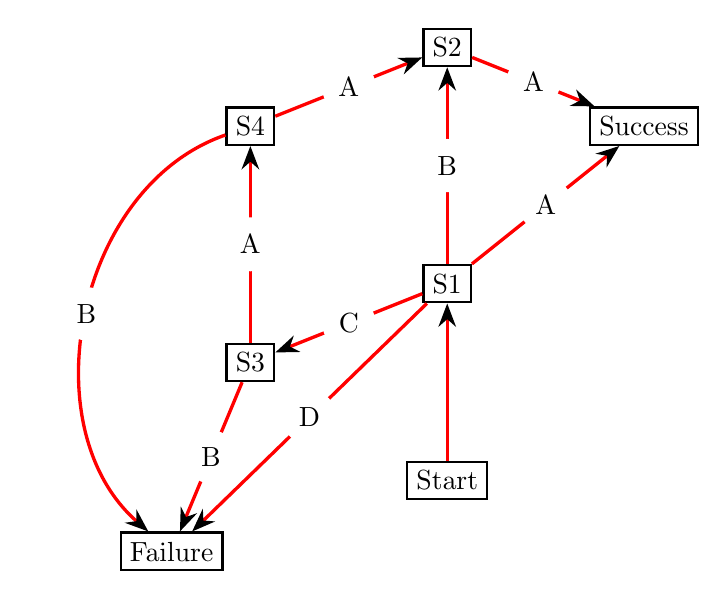
\begin{tikzpicture}
\begin{scope}[every node/.style={rectangle,thick,draw}]
    \node (A) at (0,0) {S3};
    \node (B) at (0,3) {S4};
    \node (C) at (2.5,4) {S2};
    \node (D) at (2.5,1) {S1};
    \node (E) at (2.5,-1.5) {Start};
    \node (F) at (5,3) {Success} ;
	\node (G) at (-1, -2.4) {Failure};
\end{scope}

\begin{scope}[>={Stealth[black]},
              every node/.style={fill=white,circle},
              every edge/.style={draw=red,very thick}]
    \path [->] (A) edge node {A} (B);
    \path [->] (B) edge node {A} (C);
    \path [->] (D) edge node {C} (A);
    \path [->] (D) edge node {B} (C);
    \path [->] (A) edge node {B} (G);
    \path [->] (D) edge node {D} (G);
    \path [->] (D) edge node {A} (F);
    \path [->] (C) edge node {A} (F);
    \path [->] (E) edge (D);
    \path [->] (B) edge[bend right=60] node {B} (G);
\end{scope}
\end{tikzpicture}
\caption{A depiction of the relationship between scenes using a graph representation. Adapted from~\cite{tAnswerDrawGraph2015}}\label{fig:scene_graph}
\end{figure}
The graph representation of scenes will serve as a replacement for the preview panel. Instead of providing a text based representation of the relationships between scenes, consider providing a visual one such as displayed in figure \ref{fig:scene_graph}. A popular example comes from Obsidian's knowledge graph~\cite{ObsidianSharpenYour}, which contains back-links and grouping to visually demonstrate the relationship between different nodes in the graph.

An automatically generated graph could easily be produced from the data in a scene, but rendering the graph would take some engineering, hence the predicted time alottment.

In addition to allowing the user control over the way their scenes interact and providing more detailed information on the scenario structure, this also adds an option for a new type of node creation that could be done visually in the graph. This, though an interesting idea, we leave cost-benefit analysis to the reader.

\section{Conclusion}
Through the course of this paper, we identify a number of visual, functional and documentation problems throughout the Illumia Labs \textit{Scenario Builder}. We find that the user interface is hard to navigate and invites unnecessary interaction, detracting from the ease of use of the program through aspects such as colour scheme, layout, alignment and contrast, as well as a number of Gestalt principles detailed in section \ref{sec:flaws}. We then propose a five-step plan to correct the presented issues and discuss potential solutions for each identified problem. We expand on some problems with the current UI in the appendix, and discuss the reasons we suggest doing a complete revamp of the UI. Our analysis cites both the literature and popular implementation practices used by the community to provide insight in making the Illumia Labs \textit{Scenario Builder} a more attractive and user-friendly application.

\section{Acknowledgments}
We would like to acknowledge the help of our wonderful TA's and professor for guiding us on this journey.

% bibliography data
\bibliographystyle{ACM-Reference-Format}
\bibliography{bibliography}

\section*{Appendices}
%%
%% If your work has an appendix, this is the place to put it.
\appendix

\section{Notes on the Current UI}
We found a number of significant problems with the current UI, leading us to suggest a complete revamp of the frontend of the application. The first of which is the navigation pain, as discussed in section \ref{remediations}, but particularly the lack of useful information provided in any given program state. One way to fix this would be to use the loading screens as a form of tutorial, teaching the user how to perform tasks in the program, but as stated above, there is too much useless interaction with the home pages.

Currently, the program also fails to offer a `dashboard-esque' area for clients to view their created scenes or get a feel for the global structure of their scenario. We did not identify an easy way to solve this problem in the current UI paradigm, despite the implementation of a preview pane. Additionally, there are misleading interactions in the current UI caused by a clash between the classical implementation of the tab-bar and the implementation presented in the \textit{Scenario Builder}, such as the arrow buttons (which we initially expect to move us between tabs) and the drop-down-delete menu that could be moved into the tab itself.

With the number of problematic features in the tab-bar paradigm and the community's current affinity for the sidebar, we suggest a re-implementation of the front end using the sidebar paradigm presented in the paper.


\section{Additional Functionality issues}
During our evaluation, we encountered a number of indicated features (in addition to the saving and avatar) that were not implemented or whose implementation was questionable. We present a discussion of each element in depth here.

\subsection{AI Features}
\subsubsection{Suggest Prompt}
The suggest prompt option in the scene creation menu creates a prompt seemingly from a writing prompt, and not from the business orientation that we observed in our trial of the system. Improving the prompt engineering in the API call will likely solve this problem. This particular action provides no visual queue to confirm that it has executed, which causes some confusion and may make users suspect it is broken.

\subsubsection{Suggest Transition}
The suggest transition button on the same screen as the suggest prompt button has no appreciable effect.

\subsection{Quality of Life features}
\subsubsection{Deletion}
The option to delete tabs is somewhat cryptic since it deletes tabs in numerical order, while maintaining a complete number line. This couples with user inability to change the name of a scene, which is a significant problem.

\subsubsection{Debugging}
The current messages to users that a scene or option is invalid only recognizes the first error. Such error mitigation indicators should find all errors before terminating to give the user a better idea of all areas in need of change.

\subsection{Avatar Builder Issues}
\subsubsection{Avatar URL}
Manual entry for avatar URL is confusing and lacks guidance on obtaining a URL. Additionally, the avatar URL entry sometimes fails to appear for input.

\subsubsection{Saving the Avatar}
The 'Next' button does not save the avatar, misleading the user.

\subsubsection{Language Selector}
Language selection issues in the avatar builder, this presents a strange bug where users are redirected unexpectedly to the outfit section of the builder when they decide to change their language. This language change also fails to translate many UI elements into the target language.

\subsubsection{Exporting Avatars}
Lack of export or save option for avatars. There is a need for a proper saving functionality, perhaps including unique avatar creation IDs, incorporating an account-like system.

\section{Positive Notes}
With the amount of criticism we do for these types of systems, it is important to note the positive aspects of a given system. The driving idea for this system has great potential, the use of virtual and augmented reality presents opportunities never before excersized for training and risk-free orientations to complex systems. This system presents an interesting angle of attack for the industry, and with proper implementation of machine learning tools the training opportunities and candidate evaluation techniques available will increase greatly.
\end{document}
\endinput
%%
%% End of file `sample-lualatex.tex'.

% LocalWords:  alottment paralell excersized
